\documentclass{article}
\usepackage[utf8]{inputenc}
\usepackage{authblk} % To make the adress/email look ok
\usepackage{amsmath} % To use mathematics
\usepackage{tcolorbox} % To use box around text
\usepackage{float}



\title{Labreport 1}
\author{Mohammad Abdulsalam Hajjo}
\affil{Perspectives on Computer Science and Engineering, Group 3, mohhaj21@student.hh.se}
\date{October 2020}

\begin{document}

\maketitle

\section{Introduction}
This lab is for us to learn how to import data into Matlab and how to plot them. In addition this lab is for us to learn how to call functions that are built in Matlab, such as, ttest2. 
\section{Task 1}
Basiclly the first task is about importing data from a zip file where each student have their own file to import. 

\subsection{Code}
\begin{tcolorbox}
\begin{verbatim}
load Person_139.mat
plot(Person_139.run,'.','color', 'g');
hold on
plot(Person_139.rest,'.','color', 'k')
xlabel('Days','FontSize', 14); 
ylabel('Pulses','FontSize', 14);
legend('walking','Runing')
hold off
\end{verbatim}
\end{tcolorbox}

\subsection{Task 1 result}
\begin{figure}[H]
\centering
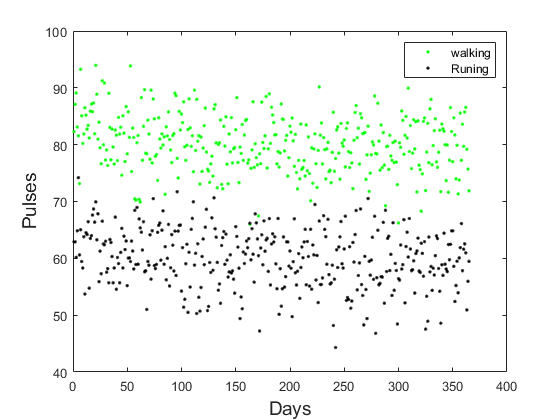
\includegraphics[angle=0,width=8cm]{Lab1_figure1.png}
\caption{Plot results}
\label{fig:circleAndSquareArea}
\end{figure}

\section{Task 2}
Task 2 is about using a built in function to investigate if the person has improved their heart rate after 6months of exercising. 
\subsection{Code}
\begin{tcolorbox}
\begin{verbatim}
rest_first_half = Person_139.rest(1:182);
rest_second_half = Person_139.rest(183:365);
[h,p] = ttest2(rest_first_half, rest_second_half);
\end{verbatim}
\end{tcolorbox}

\subsection{Task 2 result}
The code have been used and gave the following result, that the H value equals 1, and the P value equals 1.893504638018083e-04. We can say that the H value means that there is a difference between the first and second half of the year. Because our P value is so small value so we can say that there is a small Chance that our H value is wrong. 

\newpage
\section{Tail function}
In order to compare the given values, the built in function (Tail) were used and gave h and p value. The Tail function gave us a new H and P values. The H value = 1 and the p value = 9.467523190090416e-05 which also mean 0.0000946.\\
\\We can consider the P value as how much we are confident that our null hypothesis is true. The null hypothesis is that there is no difference between x and y, so they belong to the same underline distribution. When our null hypothesis is true our H value is zero, therefore we accept the null hypothesis. The maximum P value we can get is 1, and it then that means we are absolutely certain that x and y belong to the same underline distribution, so we do not reject the null hypothesis.\\
\\In our case we can see that our p value is very very small, so we are not at all confident that our null hypothesis is true, which means that the alternative hypothesis is true, that they are different. We only reject the null hypothesis if the P value is less than 5 percent (0,05). Because my P value (0.0000946) is less than 5 percent, that is why our H value is 1, so I am rejecting the null hypothesis that they are from the same underline distribution.

\subsection{Code}
\begin{tcolorbox}
\begin{verbatim}
[h,p] = ttest2(rest_first_half, rest_second_half, 'Tail', 'right');
\end{verbatim}
\end{tcolorbox}
In other words, cause our new H value equals 1, we can say that the value of the first half of the year is bigger than the second half, which in this case mean that the person 139 breathing got better. 






\end{document}
